\documentclass[11pt,a4paper]{article}
\usepackage[T1]{fontenc}
\usepackage[utf8]{inputenc}
\usepackage{mathpazo}
\usepackage[scaled=0.92]{helvet}
\usepackage[a4paper,margin=2.3cm]{geometry}
\usepackage{graphicx,booktabs,tabularx,array,float,amsmath,xcolor,enumitem,microtype}
\usepackage[font=small,labelfont=bf,skip=4pt]{caption}
\usepackage{titlesec,fancyhdr}
\usepackage[colorlinks=true,linkcolor=navy,urlcolor=navy]{hyperref}

% --- Français : babel si disponible, sinon libellés traduits à la main ---
\IfFileExists{french.ldf}{\usepackage[french]{babel}}{%
  \renewcommand{\contentsname}{Table des matières}
  \renewcommand{\figurename}{Figure}
  \renewcommand{\tablename}{Tableau}
  \renewcommand{\refname}{Références}
  \renewcommand{\abstractname}{Résumé}
  \frenchspacing}

\definecolor{navy}{HTML}{1F3A5F}
\graphicspath{{../outputs/figures/}}
\titleformat{\section}{\Large\bfseries\sffamily\color{navy}}{\thesection}{0.6em}{}
\titleformat{\subsection}{\large\bfseries\sffamily\color{navy}}{\thesubsection}{0.6em}{}
\titlespacing*{\section}{0pt}{14pt}{6pt}
\titlespacing*{\subsection}{0pt}{10pt}{4pt}
\setlength{\parskip}{5pt}\setlength{\parindent}{0pt}
\setlist{itemsep=1pt,topsep=3pt,leftmargin=1.4em}
\hyphenpenalty=4000 \tolerance=2500 \emergencystretch=2em
\pagestyle{fancy}\fancyhf{}
\fancyhead[L]{\small\sffamily Segmentation de clientèle bancaire}
\fancyhead[R]{\small\sffamily Master BDA/IA --- UN-CHK}
\fancyfoot[C]{\small\thepage}
\renewcommand{\headrulewidth}{0.3pt}
\newcolumntype{L}[1]{>{\raggedright\arraybackslash}p{#1}}
\renewcommand{\arraystretch}{1.25}
\newcolumntype{Y}{>{\raggedright\arraybackslash}X}

\begin{document}

% ------------------------------------------------------------------ Titre
\thispagestyle{empty}
\begin{center}
{\sffamily\small Université Numérique Cheikh Hamidou Kane (UN-CHK) --- Master BDA/IA\\
Module « Apprentissage non supervisé » --- Projet final}\\[1.1cm]
{\sffamily\bfseries\huge\color{navy} Segmentation de clientèle bancaire\\[4pt]
par apprentissage non supervisé}\\[0.5cm]
{\large Jeu de données \emph{Bank Marketing} (UCI)}\\[0.9cm]
{\large Ndeye Sokhna Nokho}\\[4pt]
{\normalsize Enseignant : M. Cheikh GUEYE}\\[4pt]
{\small Octobre 2026}
\end{center}
\vspace{0.4cm}

\begin{abstract}\noindent
Une banque souhaite cibler ses campagnes de marketing téléphonique, sans disposer d'aucune segmentation de ses clients. À partir de 41\,176 contacts décrits par des variables numériques et catégorielles, nous comparons neuf méthodes de clustering (K-means, K-medoids, K-prototypes, mélange gaussien, classification hiérarchique avec quatre liens, DBSCAN) sur deux représentations des données et plusieurs mesures de dissimilarité, dont la distance de Gower. Les partitions sont évaluées par des indices internes (silhouette, Davies-Bouldin, Dunn), externes (ARI, NMI, V-mesure) et par une étude de stabilité. La solution retenue, choisie sur les seuls indices internes et la stabilité, est une classification hiérarchique de Ward à quatre segments (silhouette 0,21 ; ARI bootstrap 0,93). Le taux de souscription varie de 5\,\% à 41\,\% selon le segment, alors que cette information n'a servi ni à construire ni à choisir les groupes : en appelant un tiers des clients, la banque obtiendrait environ deux tiers des souscriptions. Deux extensions complètent l'étude : une analyse de sensibilité au contexte économique et la détection des clients atypiques (DBSCAN, Isolation Forest).
\end{abstract}

\vspace{0.2cm}
\setcounter{tocdepth}{1}
{\small\tableofcontents}
\newpage

% ------------------------------------------------------------------ 1
\section{Introduction}

Le marketing téléphonique coûte cher : chaque appel mobilise un conseiller, et la grande majorité des appels n'aboutit pas. Dans le jeu de données étudié, seuls 11\,\% des contacts se terminent par la souscription d'un dépôt à terme. Appeler tout le monde de la même façon revient donc à gaspiller neuf appels sur dix.

L'objectif du projet est de \textbf{découvrir des groupes de clients homogènes}, sans utiliser l'information de souscription, puis de vérifier que ces groupes ont un sens pour la banque. Il s'agit d'un problème d'apprentissage \emph{non supervisé} : aucune étiquette ne guide les algorithmes. La variable de souscription \texttt{y} est mise de côté dès le chargement et ne sert qu'à l'évaluation finale.

Trois questions structurent le travail :
\begin{enumerate}
\item Comment mesurer la ressemblance entre deux clients quand les données mélangent des nombres et des catégories ?
\item Quelle méthode de clustering et quel nombre de groupes retenir ?
\item Les segments obtenus sont-ils stables, interprétables et utiles pour le ciblage ?
\end{enumerate}

Le rapport suit le déroulement du projet : données et préparation (section~\ref{sec:donnees}), méthodologie (section~\ref{sec:methodo}), résultats (section~\ref{sec:resultats}), interprétation métier (section~\ref{sec:metier}), extensions (section~\ref{sec:extensions}), puis discussion et conclusion. L'ensemble du code est fourni sous forme de six notebooks exécutables de bout en bout, avec une graine aléatoire fixée, et d'une petite application Streamlit.

% ------------------------------------------------------------------ 2
\section{Données et préparation}\label{sec:donnees}

\subsection{Le jeu de données}
Le fichier \texttt{bank-additional-full.csv} (UCI Machine Learning Repository) contient 41\,188 contacts téléphoniques d'une banque portugaise, décrits par 20 variables et la cible \texttt{y}. Les variables se répartissent en quatre familles : le \textbf{profil du client} (âge, profession, statut marital, niveau d'études, crédits), la \textbf{campagne en cours} (canal, mois, jour, durée et nombre d'appels), l'\textbf{historique} (contacts et résultat de la campagne précédente) et le \textbf{contexte économique} (cinq indicateurs trimestriels ou mensuels). Dix variables sont numériques, dix sont catégorielles : les données sont \emph{mixtes}.

\subsection{Nettoyage}
\begin{itemize}
\item \textbf{Doublons} : 12 lignes strictement identiques sont supprimées (41\,176 clients restants).
\item \textbf{Valeurs manquantes} : elles sont codées par la modalité \texttt{unknown}. Pour \texttt{job}, \texttt{marital}, \texttt{education}, \texttt{housing} et \texttt{loan} (moins de 5\,\% de cas), on impute le mode. Pour \texttt{default}, \texttt{unknown} représente 21\,\% des clients : on la conserve comme modalité, car ne pas connaître la situation de défaut est une information en soi.
\item \textbf{Valeurs aberrantes} : \texttt{campaign} a une queue très longue (jusqu'à 56 appels) ; elle est plafonnée au 99\textsuperscript{e} centile (14 appels). Les âges élevés sont de vrais clients et sont conservés. Dans \texttt{pdays}, la valeur 999 est un code signifiant « jamais recontacté » : la variable est remplacée par l'indicateur binaire \texttt{contacted\_before}.
\end{itemize}

\subsection{Variables actives et variables illustratives}
Toutes les variables ne doivent pas servir à construire les groupes. Nous distinguons les variables \emph{actives}, utilisées par les algorithmes, des variables \emph{illustratives}, écartées du calcul mais conservées pour décrire les segments (tableau~\ref{tab:roles}).

\begin{table}[H]\centering\small
\caption{Variables écartées du clustering et justification.}\label{tab:roles}
\begin{tabularx}{\textwidth}{|L{3.6cm}|Y|}
\hline
\textbf{Variable} & \textbf{Raison de l'exclusion}\\ \hline
\texttt{duration} & Connue seulement après l'appel, donc inutilisable pour cibler à l'avance ; de plus presque déterminante pour \texttt{y} (un appel de 0~s donne toujours \texttt{no}).\\ \hline
\texttt{emp.var.rate}, \texttt{nr.employed} & Corrélées à plus de 0,90 avec \texttt{euribor3m} (figure~\ref{fig:corr}) : les garder compterait trois fois la même information dans les distances.\\ \hline
\texttt{month}, \texttt{day\_of\_week} & Décrivent le calendrier de la campagne, pas le client.\\ \hline
\texttt{pdays} & Recodée en \texttt{contacted\_before}.\\ \hline
\end{tabularx}
\end{table}

Il reste \textbf{15 variables actives} : six numériques (\texttt{age}, \texttt{campaign}, \texttt{previous}, \texttt{cons.price.idx}, \texttt{cons.conf.idx}, \texttt{euribor3m}) et neuf catégorielles (\texttt{job}, \texttt{marital}, \texttt{education}, \texttt{default}, \texttt{housing}, \texttt{loan}, \texttt{contact}, \texttt{poutcome}, \texttt{contacted\_before}).

\begin{figure}[H]\centering
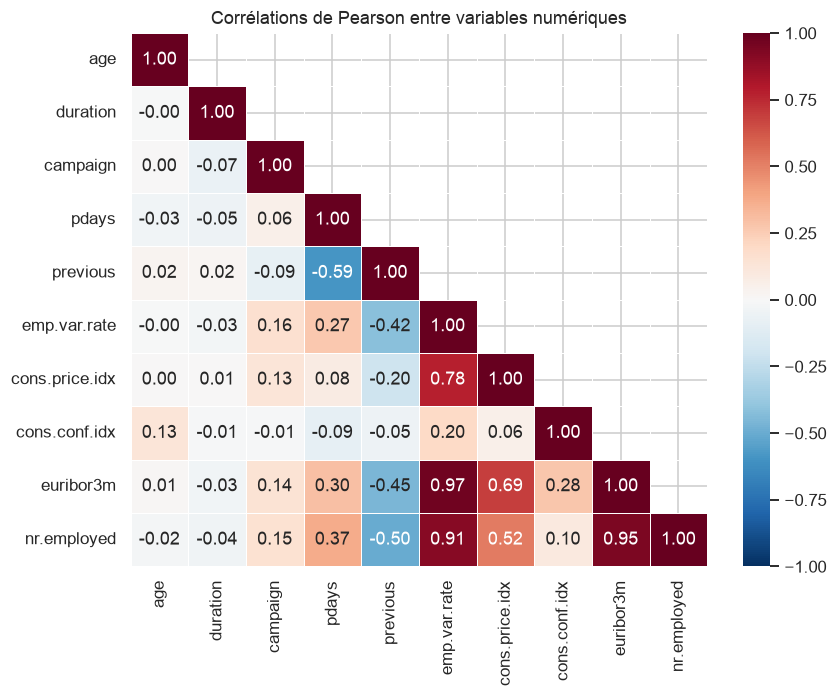
\includegraphics[width=0.60\textwidth]{01_correlations.png}
\caption{Corrélations entre variables numériques. Trois indicateurs économiques sont presque redondants.}\label{fig:corr}
\end{figure}

\subsection{Deux représentations et un échantillon}
Deux représentations sont construites par une fonction réutilisable (\texttt{prepare\_all}) :
\begin{itemize}
\item \textbf{(a) one-hot + standardisation} : indicatrices 0/1 pour les catégories, variables numériques centrées-réduites $z=(x-\mu)/\sigma$. Elle compte 37 colonnes et sert aux méthodes euclidiennes.
\item \textbf{(b) données mixtes brutes} : 15 colonnes dans leur nature d'origine, pour la distance de Gower et K-prototypes.
\end{itemize}

Les méthodes à matrice de distances stockent $n^2$ valeurs. Elles sont donc appliquées à un \textbf{échantillon aléatoire stratifié de 4\,000 clients}. La stratification porte sur \texttt{y} uniquement pour conserver le taux de souscription de la population (11,3\,\%) ; aucun algorithme ne voit cette variable. Les moyennes de l'échantillon s'écartent de moins de 5\,\% de celles de la population.

\subsection{Réduction de dimension}
L'analyse en composantes principales montre une variance très répartie : le premier plan n'en conserve que 36\,\% (23,5\,\% et 12,8\,\%) et il faut 10 composantes pour atteindre 80\,\%. Le premier axe oppose le contexte économique (\texttt{euribor3m}, \texttt{cons.price.idx}) à l'historique de contact (\texttt{previous}) ; le second est porté par l'âge et la confiance des ménages.

Les projections non linéaires t-SNE et UMAP (figure~\ref{fig:proj}) font apparaître quelques îlots, liés au niveau des taux et à l'historique de contact, mais pas trois ou quatre « boules » nettement séparées. On s'attend donc à des clusters qui se chevauchent.

\begin{figure}[H]\centering
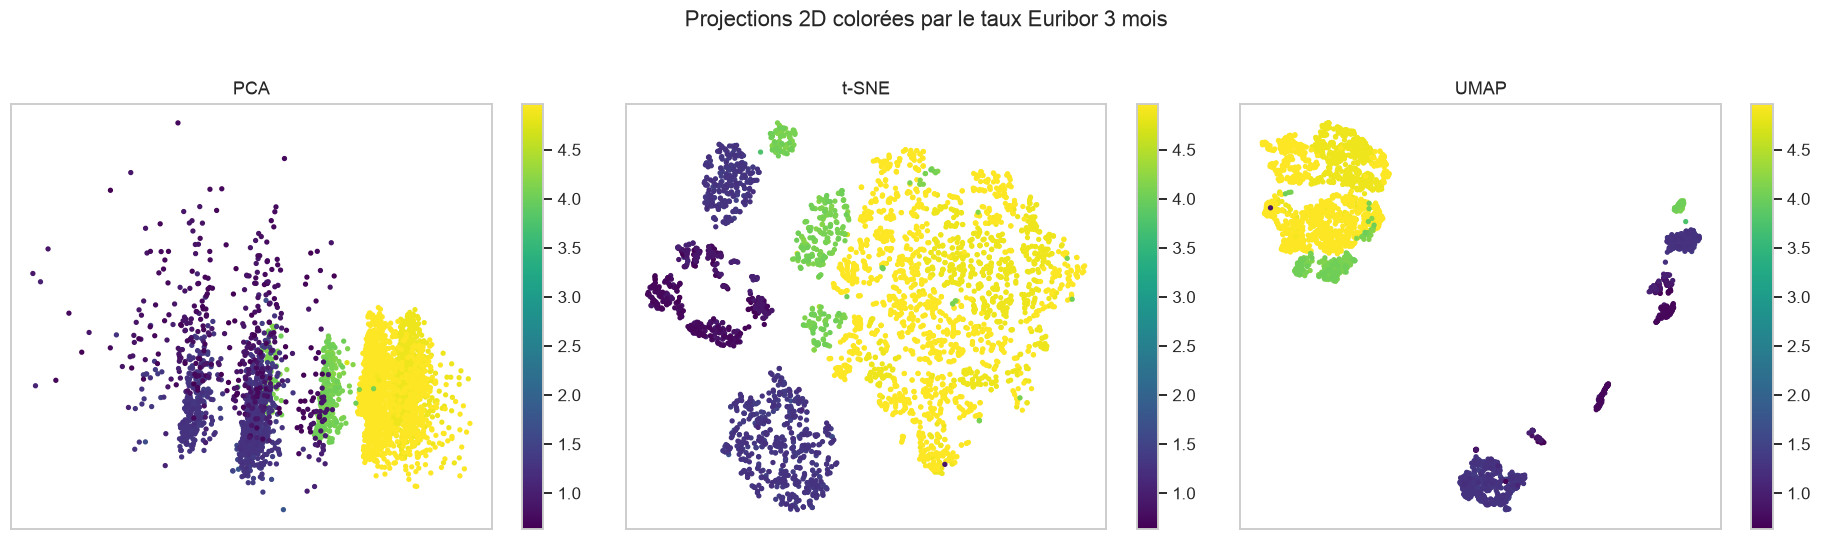
\includegraphics[width=\textwidth]{01_projections_euribor.png}
\caption{Projections en deux dimensions de l'échantillon, colorées par le taux Euribor à 3 mois.}\label{fig:proj}
\end{figure}

% ------------------------------------------------------------------ 3
\section{Méthodologie}\label{sec:methodo}

\subsection{Mesures de dissimilarité}
Cinq mesures sont calculées et comparées :
\begin{itemize}
\item \textbf{euclidienne} et \textbf{Manhattan} sur la représentation (a), avec et sans standardisation ;
\item \textbf{Hamming} et \textbf{Jaccard} sur le bloc des variables binaires. Hamming compte de la même façon les accords « oui-oui » et « non-non » : elle convient aux variables symétriques (canal de contact). Jaccard ignore les accords « non-non » : elle convient aux variables asymétriques, où le « oui » est rare (succès à la campagne précédente : 3\,\% des clients) ;
\item \textbf{Gower} sur la représentation (b) :
\[
d(x,x') = \frac{1}{p}\sum_{j=1}^{p} d_j(x_j,x'_j),\qquad
d_j=\begin{cases}\dfrac{|x_j-x'_j|}{\text{étendue}_j} & \text{si $j$ est numérique}\\[8pt] \mathbf{1}[x_j\neq x'_j] & \text{si $j$ est catégorielle.}\end{cases}
\]
Chaque variable contribue entre 0 et 1 : toutes ont le même poids, quel que soit leur type.
\end{itemize}

\subsection{Méthodes de clustering}
Le tableau~\ref{tab:methodes} résume les méthodes mises en œuvre et la distance associée à chacune.

\begin{table}[H]\centering\small
\caption{Méthodes de clustering comparées.}\label{tab:methodes}
\begin{tabularx}{\textwidth}{|L{2.9cm}|L{3.3cm}|Y|}
\hline
\textbf{Méthode} & \textbf{Données / distance} & \textbf{Principe et réglage}\\ \hline
K-means & (a), euclidienne & Minimise l'inertie intra-classe ; 10 initialisations ; $k$ de 2 à 10 (méthode du coude).\\ \hline
K-medoids & matrice de Gower & Le centre est un client réel (médoïde) ; fonctionne avec toute dissimilarité.\\ \hline
K-prototypes & (b), mixte & Moyenne pour les numériques, mode pour les catégorielles.\\ \hline
Mélange gaussien & 10 axes de la PCA & Affectation probabiliste, clusters elliptiques ; critères BIC et AIC.\\ \hline
CAH (4 liens) & (a), euclidienne & \emph{Single}, \emph{complete}, \emph{average}, Ward ; coupure choisie sur le dendrogramme.\\ \hline
CAH lien moyen & matrice de Gower & Variante adaptée aux données mixtes.\\ \hline
DBSCAN & 5 axes de la PCA & Clusters = zones denses ; $\varepsilon$ réglé par le graphique des $k$-distances, \texttt{min\_samples} = 10.\\ \hline
\end{tabularx}
\end{table}

\textbf{Remarque d'implémentation.} La bibliothèque \texttt{scikit-learn-extra}, indiquée dans le sujet pour K-medoids, n'est plus maintenue et ne s'importe pas avec NumPy~2. Le code l'utilise si elle est disponible et bascule sinon sur une implémentation personnelle du même algorithme (alternance affectation / mise à jour des médoïdes, initialisation de type \emph{k-medoids++}).

\subsection{Validation}
\begin{itemize}
\item \textbf{Indices internes} : silhouette (entre $-1$ et 1, à maximiser), Davies-Bouldin (à minimiser) et Dunn (à maximiser ; implémentation personnelle). La silhouette est calculée dans l'espace euclidien \emph{et} en distance de Gower, pour ne favoriser aucune famille de méthodes.
\item \textbf{Indices externes} par rapport à \texttt{y} : ARI, NMI, homogénéité, complétude, V-mesure.
\item \textbf{Stabilité} : K-means relancé avec 20 graines (une seule initialisation) ; puis 20 rééchantillons bootstrap, en mesurant l'ARI entre la partition de référence et la partition obtenue sur chaque rééchantillon.
\end{itemize}

% ------------------------------------------------------------------ 4
\section{Résultats}\label{sec:resultats}

\subsection{Effet de la standardisation et choix des distances}
Sans standardisation, l'âge porte à lui seul \textbf{77\,\%} de la distance euclidienne, simplement parce qu'il s'exprime en dizaines d'unités (figure~\ref{fig:poids}). Après standardisation, chaque variable numérique pèse environ 10\,\% et les variables catégorielles retrouvent une influence. L'effet sur les voisinages est massif : seuls 23\,\% des dix plus proches voisins d'un client restent les mêmes. À l'inverse, euclidienne et Manhattan standardisées partagent 83\,\% de leurs voisins : le choix entre ces deux distances a peu d'effet.

\begin{figure}[H]\centering
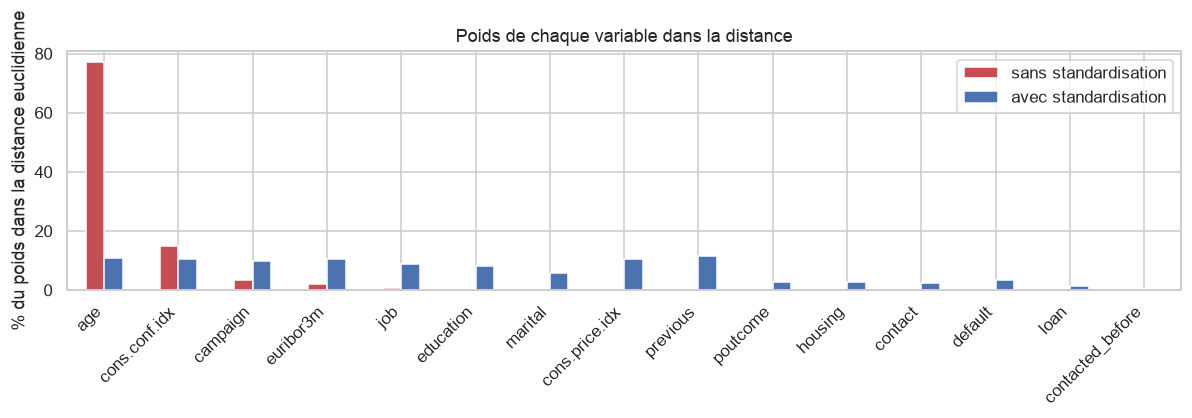
\includegraphics[width=0.86\textwidth]{02_poids_variables.png}
\caption{Poids de chaque variable dans la distance euclidienne, sans et avec standardisation.}\label{fig:poids}
\end{figure}

Nous retenons donc la distance euclidienne \emph{standardisée} pour les méthodes qui reposent sur des moyennes (K-means, mélange gaussien, Ward, DBSCAN), et la distance de \textbf{Gower} pour celles qui acceptent une dissimilarité quelconque (K-medoids, CAH à lien moyen). Gower corrige le défaut restant de la représentation (a), qui place arbitrairement sur la même échelle un écart-type d'âge et un changement de modalité.

\subsection{Méthodes de partitionnement}
Pour K-means, la courbe d'inertie décroît sans cassure franche (figure~\ref{fig:coude}). Chaque groupe ajouté fait gagner 7 à 9\,\% d'inertie jusqu'à $k=6$, puis moins de 4\,\% : le coude se situe vers $k=6$. La silhouette, elle, est maximale pour $k=2$ (0,24), reste proche de 0,20 jusqu'à $k=5$, puis chute. Les deux critères encadrent le choix sans le trancher.

\begin{figure}[H]\centering
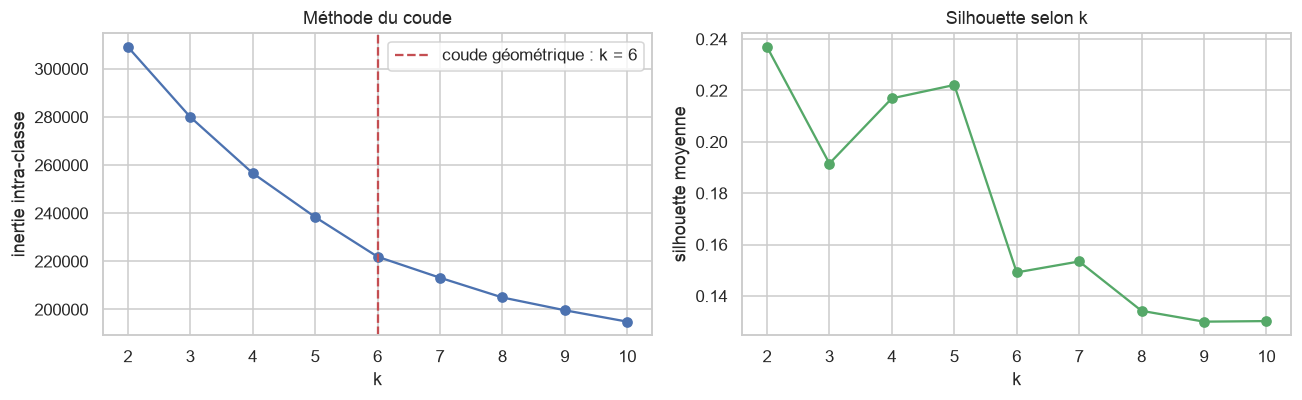
\includegraphics[width=0.92\textwidth]{02_kmeans_coude.png}
\caption{K-means sur la population complète : inertie et silhouette en fonction de $k$.}\label{fig:coude}
\end{figure}

\begin{table}[H]\centering\small
\caption{Méthodes de partitionnement sur l'échantillon (silhouette : plus haut = mieux ; Davies-Bouldin : plus bas = mieux).}\label{tab:partition}
\begin{tabular}{|l|c|c|c|c|c|}
\hline
\textbf{Méthode} & $k$ & \textbf{Silh. eucl.} & \textbf{Silh. Gower} & \textbf{Davies-B.} & \textbf{Plus petit cluster}\\ \hline
K-means            & 2 & 0,237 & 0,233 & 1,88 & 33,8\,\%\\ \hline
K-means            & 3 & 0,186 & 0,175 & 1,92 & 14,3\,\%\\ \hline
K-means            & 4 & 0,182 & 0,121 & 1,84 & 7,9\,\%\\ \hline
K-medoids (Gower)  & 2 & 0,111 & 0,180 & 2,54 & 45,5\,\%\\ \hline
K-medoids (Gower)  & 3 & 0,039 & 0,111 & 3,73 & 26,8\,\%\\ \hline
K-prototypes       & 2 & 0,236 & 0,232 & 1,88 & 33,8\,\%\\ \hline
K-prototypes       & 3 & 0,185 & 0,175 & 1,92 & 14,3\,\%\\ \hline
K-prototypes       & 4 & 0,126 & 0,089 & 2,26 & 7,6\,\%\\ \hline
Mélange gaussien   & 2 & 0,235 & 0,233 & 1,89 & 34,6\,\%\\ \hline
Mélange gaussien   & 3 & 0,078 & 0,127 & 3,16 & 30,0\,\%\\ \hline
\end{tabular}
\end{table}

Trois constats ressortent du tableau~\ref{tab:partition} :
\begin{itemize}
\item \textbf{À $k=2$, K-means, K-prototypes et le mélange gaussien trouvent la même coupure} (ARI entre partitions supérieur à 0,97) : les clients contactés en période de taux élevés contre ceux contactés en période de taux bas.
\item À $k=3$, K-means et K-prototypes restent d'accord (ARI = 0,99) et isolent un groupe de clients déjà démarchés. À $k=4$, en revanche, K-prototypes devient sensible à l'initialisation : une ré-exécution dans un autre environnement logiciel, à graine égale, donne une partition très différente (ARI de 0,51 avec la précédente). K-means présente la même fragilité à $k=4$ (section~\ref{sec:valid}). Le mélange gaussien découpe autrement, avec des indices nettement moins bons. Son BIC décroît d'ailleurs jusqu'à $k=10$ sans minimum net : les données, faites d'indicatrices et d'indicateurs prenant peu de valeurs, sont loin d'être gaussiennes, et le BIC ne peut pas servir seul à choisir $k$.
\item \textbf{K-medoids sur Gower} donne une structure faible (silhouette de Gower autour de 0,11) et des groupes très différents des autres méthodes (ARI de 0,18 avec K-means). Comme Gower donne le même poids aux 15 variables, le contexte économique ne domine plus et les groupes se forment sur d'autres critères (canal, prêt immobilier, statut marital).
\end{itemize}

\subsection{Classification hiérarchique}
Le choix du lien change entièrement le résultat (tableau~\ref{tab:liens}). Le lien \emph{single} produit un effet de chaîne : un cluster géant et des singletons. Les liens \emph{average} et \emph{complete} isolent quelques dizaines de clients atypiques. Seul le lien de \textbf{Ward} donne des groupes équilibrés.

\begin{table}[H]\centering\small
\caption{CAH à trois clusters selon le lien (distance euclidienne, 4\,000 clients).}\label{tab:liens}
\begin{tabular}{|l|l|c|c|}
\hline
\textbf{Lien} & \textbf{Tailles des clusters} & \textbf{Silhouette} & \textbf{Corrélation cophénétique}\\ \hline
\emph{Single}   & 3\,998 / 1 / 1     & 0,423 & 0,70\\ \hline
\emph{Complete} & 3\,879 / 66 / 55   & 0,316 & 0,75\\ \hline
\emph{Average}  & 3\,964 / 35 / 1    & 0,489 & 0,83\\ \hline
Ward            & 2\,617 / 756 / 627 & 0,193 & 0,58\\ \hline
\end{tabular}
\end{table}

Ce tableau illustre un piège : les trois liens inutilisables affichent les \emph{meilleures} silhouettes. Isoler une poignée de points très éloignés suffit à obtenir une silhouette élevée. Un indice ne se lit donc jamais sans la taille des clusters ; ce garde-fou est repris dans la sélection finale.

Le dendrogramme de Ward (figure~\ref{fig:ward}) propose deux coupures naturelles : $k=2$, de loin le plus grand saut de hauteur, et $k=5$. La silhouette classe $k=2$ en tête (0,23) puis $k=4$ (0,21) devant $k=5$ (0,18). Les partitions étant emboîtées, le grand groupe de 2\,617 clients reste intact de $k=2$ à $k=4$ ; seul l'autre groupe est subdivisé.

\begin{figure}[H]\centering
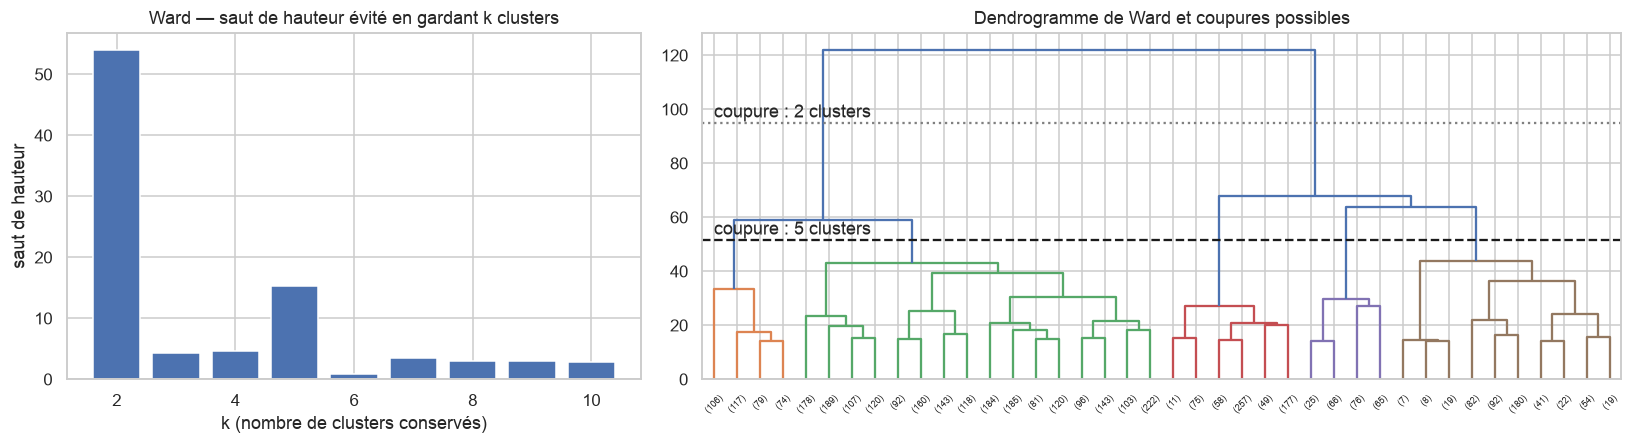
\includegraphics[width=\textwidth]{03_ward_coupure.png}
\caption{Lien de Ward : sauts de hauteur entre fusions successives et dendrogramme.}\label{fig:ward}
\end{figure}

Appliquée à la distance de Gower, la CAH à lien moyen isole des niches définies par l'historique : 130 clients dont la campagne précédente a été un succès, 482 dont elle a été un échec, et la masse des clients jamais démarchés.

\subsection{DBSCAN et limites de K-means}
Le graphique des $k$-distances donne $\varepsilon \approx 1{,}0$ pour \texttt{min\_samples} = 10. DBSCAN trouve alors 8 clusters, dont \textbf{un seul contient 82\,\% des clients}, et classe 3,8\,\% des points en bruit (figure~\ref{fig:dbscan}). Le résultat est très sensible à $\varepsilon$ : plus petit, il émiette les données ; plus grand, tout fusionne.

\begin{figure}[H]\centering
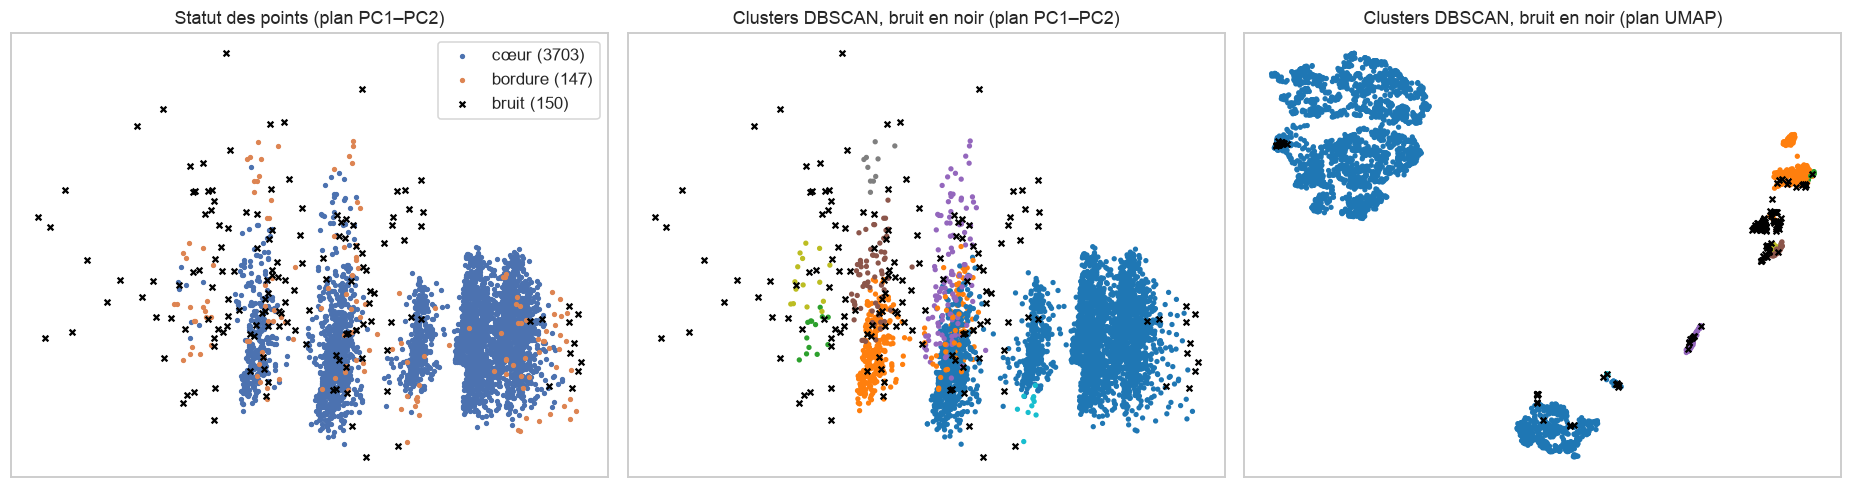
\includegraphics[width=\textwidth]{03_dbscan.png}
\caption{DBSCAN : statut des points (cœur, bordure, bruit) et clusters obtenus.}\label{fig:dbscan}
\end{figure}

La clientèle forme donc une masse continue, sans zones vides entre des groupes : DBSCAN n'est pas adapté pour la segmenter. Il est en revanche utile pour \textbf{repérer les clients atypiques}. Les points de bruit ne sont pas des erreurs : ce sont des clients plus âgés (49 ans en moyenne contre 40), déjà démarchés (42\,\% contre 2\,\%), plus souvent retraités ou étudiants (34\,\% contre 5\,\%).

Cette comparaison éclaire les limites de K-means. Ses clusters sont convexes par construction et il affecte de force chaque point à un groupe : les clients que DBSCAN classe en bruit sont, pour K-means, presque deux fois plus éloignés de leur centre que les autres (4,3 contre 2,4). Les deux méthodes sont complémentaires : l'une segmente, l'autre signale les cas atypiques.

\subsection{Validation et choix de la solution}\label{sec:valid}

\paragraph{Indices internes.} La structure la plus nette est à $k=2$ pour presque toutes les méthodes (silhouette de 0,23 à 0,24). Au-delà, Ward est la méthode qui se dégrade le moins (figure~\ref{fig:internes}). Les valeurs restent modestes : les segments se chevauchent, comme l'annonçaient les projections.

\begin{figure}[H]\centering
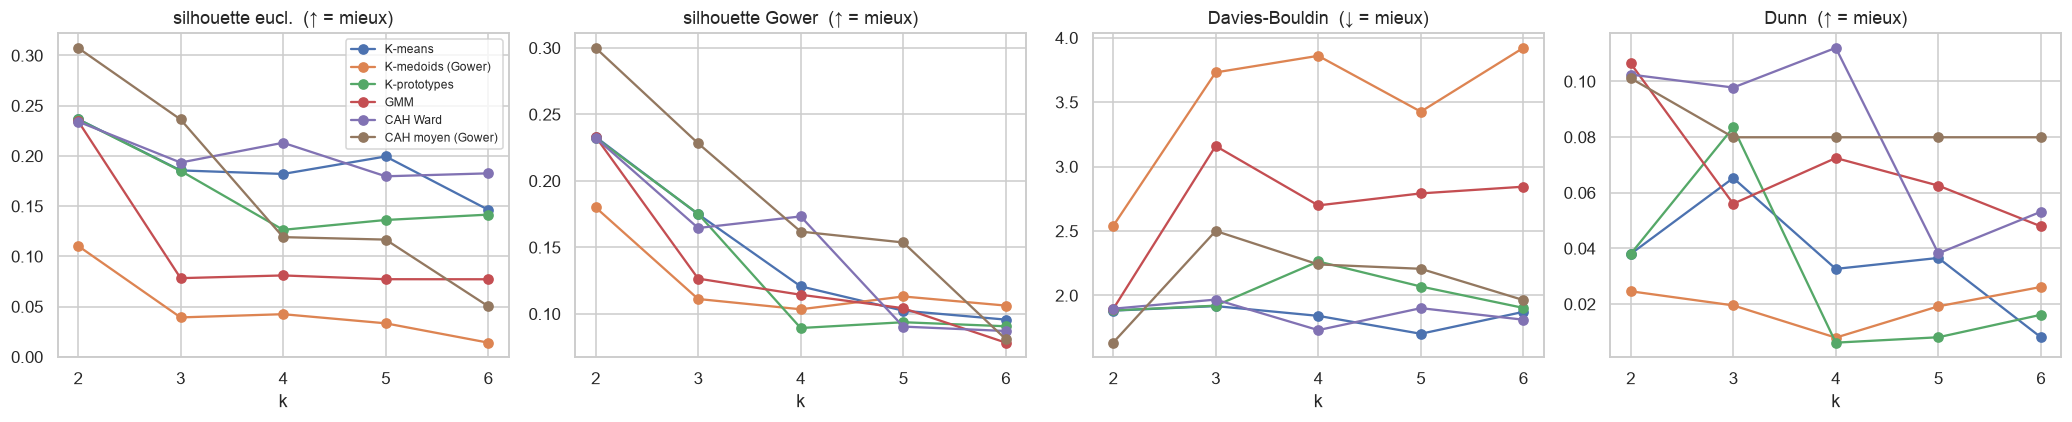
\includegraphics[width=\textwidth]{04_indices_internes.png}
\caption{Indices internes selon $k$ pour les six méthodes principales.}\label{fig:internes}
\end{figure}

\paragraph{Indices externes.} L'accord avec \texttt{y} est faible pour toutes les méthodes (ARI inférieur à 0,25). C'est attendu : \texttt{y} est binaire et très déséquilibrée, et une segmentation de clientèle n'a pas vocation à reproduire ce découpage. Les valeurs ne sont pourtant pas nulles, et surtout les taux de souscription diffèrent fortement d'un segment à l'autre (de 5\,\% à 40\,\%).

\paragraph{Stabilité.} Avec une seule initialisation, l'ARI moyen entre 20 exécutions de K-means va de 0,69 à 0,88, avec des minimums proches de 0,35 : cela justifie les 10 initialisations utilisées partout ailleurs. Le bootstrap (figure~\ref{fig:stab}) montre que K-means est très stable pour $k=2$ et $k=3$ (0,997 et 0,98), mais \textbf{instable pour $k=4$ et $k=5$} (0,72 et 0,65). Ward décroît régulièrement : 0,99, 0,96, \textbf{0,93 à $k=4$}, 0,86, 0,71.

\begin{figure}[H]\centering
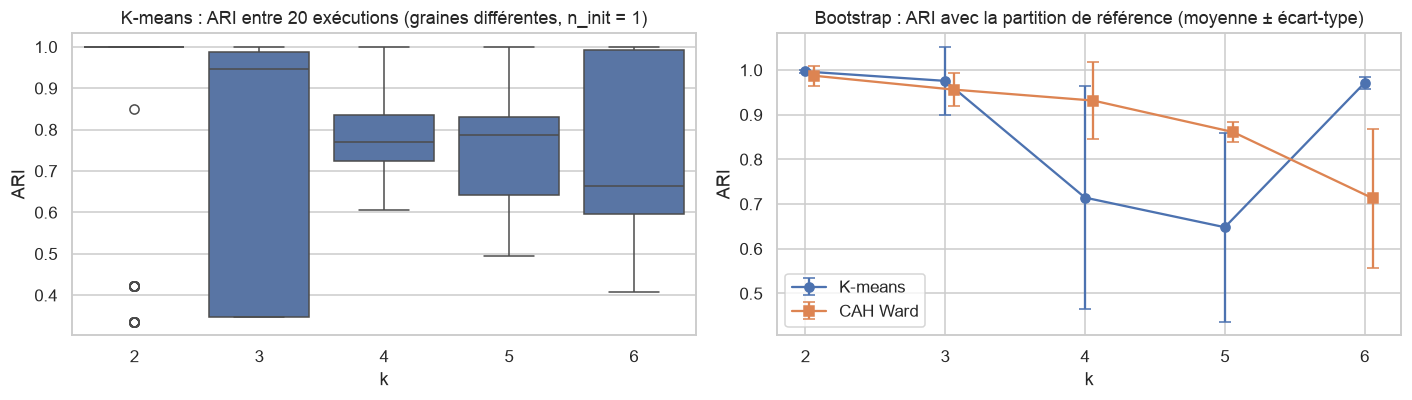
\includegraphics[width=\textwidth]{04_stabilite.png}
\caption{Stabilité : sensibilité de K-means à l'initialisation (gauche) et bootstrap pour K-means et Ward (droite).}\label{fig:stab}
\end{figure}

\paragraph{Sélection.} Elle se fait en quatre temps. (1)~Un filtre métier : le sujet demande trois à quatre recommandations, une par segment, donc $k=3$ ou 4, et chaque segment doit représenter au moins 5\,\% des clients. Ce filtre élimine les partitions déséquilibrées. (2)~Un classement des candidats sur les \textbf{quatre indices internes} seulement, résumé par leur rang moyen. (3)~Un contrôle de stabilité. (4)~Une vérification a posteriori par les indices externes. La variable \texttt{y} ne participe donc pas au choix : sinon, constater ensuite que les segments séparent bien les souscripteurs serait un raisonnement circulaire.

\begin{table}[H]\centering\small
\caption{Candidats après filtre métier, classés par rang moyen sur les quatre indices internes. L'ARI, calculé avec \texttt{y}, est affiché à titre de vérification et n'entre pas dans le rang.}\label{tab:synthese}
\begin{tabular}{|l|c|c|c|c|c|c|c|}
\hline
\textbf{Méthode} & $k$ & \textbf{Silh. eucl.} & \textbf{Silh. Gower} & \textbf{Davies-B.} & \textbf{Dunn} & \textbf{Rang moyen} & \textbf{ARI}\\ \hline
\textbf{CAH Ward}  & \textbf{4} & \textbf{0,213} & 0,173 & \textbf{1,73} & \textbf{0,112} & \textbf{1,50} & \textbf{0,151}\\ \hline
K-prototypes       & 3 & 0,185 & \textbf{0,175} & 1,92 & 0,083 & 3,00 & 0,094\\ \hline
K-means            & 3 & 0,186 & 0,175 & 1,92 & 0,065 & 3,25 & 0,096\\ \hline
CAH Ward           & 3 & 0,193 & 0,165 & 1,97 & 0,098 & 3,25 & 0,139\\ \hline
K-means            & 4 & 0,182 & 0,121 & 1,84 & 0,033 & 5,00 & 0,057\\ \hline
Mélange gaussien   & 4 & 0,081 & 0,114 & 2,70 & 0,072 & 6,25 & 0,053\\ \hline
Mélange gaussien   & 3 & 0,078 & 0,127 & 3,16 & 0,056 & 6,75 & 0,014\\ \hline
K-prototypes       & 4 & 0,126 & 0,089 & 2,26 & 0,006 & 8,00 & 0,048\\ \hline
K-medoids (Gower)  & 3 & 0,039 & 0,111 & 3,73 & 0,020 & 8,75 & 0,015\\ \hline
K-medoids (Gower)  & 4 & 0,042 & 0,103 & 3,86 & 0,008 & 9,25 & 0,002\\ \hline
\end{tabular}
\end{table}

La \textbf{CAH de Ward à quatre segments} arrive nettement en tête (tableau~\ref{tab:synthese}) : meilleure silhouette euclidienne, meilleur Davies-Bouldin et meilleur Dunn parmi les candidats, et troisième en silhouette de Gower, à 0,002 de la meilleure. Elle est aussi la plus stable : ARI bootstrap de 0,93 contre 0,72 pour K-means au même $k$. Sa silhouette (0,21) reste proche de celle de la structure à deux groupes (0,23) : on gagne deux segments sans perdre beaucoup en netteté.

Les indices externes, consultés seulement ensuite, confirment ce choix : Ward à $k=4$ a le meilleur ARI des candidats. Les ajouter au classement ne changerait pas le vainqueur.

Ce choix a un prix, qu'il faut énoncer. Statistiquement, $k=2$ reste la structure la plus nette ; $k=4$ est un choix guidé par le besoin métier et validé par les indices. Par ailleurs, Ward ne passe pas à l'échelle de la population entière : chaque client est donc affecté au segment dont le centre de gravité est le plus proche. Cette règle reproduit les segments de Ward pour 98\,\% des clients de l'échantillon.

% ------------------------------------------------------------------ 5
\section{Interprétation métier et recommandations}\label{sec:metier}

\subsection{Profil des quatre segments}
Le profilage porte sur les 41\,176 clients. Les segments sont numérotés du moins au plus souscripteur (figure~\ref{fig:taux}, tableau~\ref{tab:profils}).

\begin{figure}[H]\centering
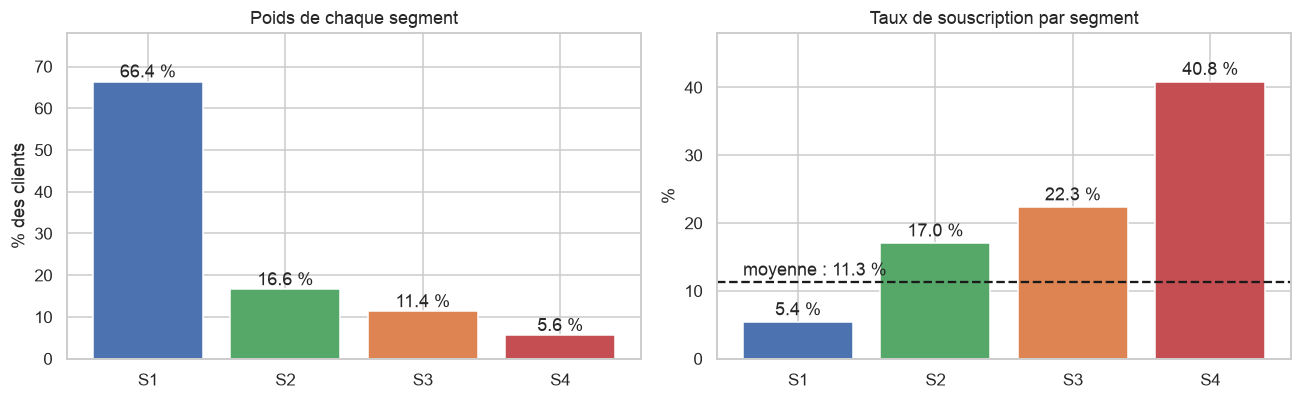
\includegraphics[width=0.88\textwidth]{05_taille_souscription.png}
\caption{Poids et taux de souscription des quatre segments.}\label{fig:taux}
\end{figure}

\begin{table}[H]\centering\small
\caption{Fiche d'identité des segments (population complète).}\label{tab:profils}
\begin{tabularx}{\textwidth}{|L{3.5cm}|Y|Y|Y|Y|}
\hline
 & \textbf{S1} & \textbf{S2} & \textbf{S3} & \textbf{S4}\\ \hline
Poids                       & 66,4\,\% & 16,6\,\% & 11,4\,\% & 5,6\,\%\\ \hline
Taux de souscription        & \textbf{5,4\,\%} & \textbf{17,0\,\%} & \textbf{22,3\,\%} & \textbf{40,8\,\%}\\ \hline
Âge moyen                   & 40,2 & 37,9 & 39,4 & 45,4\\ \hline
Appels (campagne)           & 2,7 & 2,2 & 2,0 & 1,8\\ \hline
Euribor 3 mois              & 4,8 & 1,3 & 1,6 & 0,8\\ \hline
Confiance des ménages       & $-39{,}4$ & $-46{,}0$ & $-43{,}9$ & $-30{,}7$\\ \hline
Contact sur mobile          & 50\,\% & 91\,\% & 93\,\% & 88\,\%\\ \hline
Déjà démarchés              & 0\,\% & 0\,\% & 100\,\% & 41\,\%\\ \hline
Retraités ou étudiants      & 4\,\% & 7\,\% & 9\,\% & 26\,\%\\ \hline
60 ans et plus              & 1\,\% & 3\,\% & 5\,\% & 22\,\%\\ \hline
Diplôme universitaire       & 33\,\% & 32\,\% & 34\,\% & 48\,\%\\ \hline
Défaut de crédit inconnu    & 26\,\% & 13\,\% & 12\,\% & 3\,\%\\ \hline
\end{tabularx}
\end{table}

\begin{itemize}
\item \textbf{S1 --- Nouveaux prospects, taux élevés.} Deux tiers de la clientèle. Jamais démarchés, contactés quand l'Euribor avoisine 4,8\,\%, pour moitié sur téléphone fixe. C'est le segment le plus sollicité et le moins réceptif.
\item \textbf{S2 --- Nouveaux prospects, taux bas.} Jamais démarchés non plus, mais contactés en période de taux bas, presque toujours sur mobile. Segment le plus jeune, avec 36\,\% de célibataires.
\item \textbf{S3 --- Clients déjà démarchés.} Tous ont un historique : 79\,\% d'échecs et 21\,\% de succès lors de la campagne précédente.
\item \textbf{S4 --- Profils réceptifs.} Petit segment, le plus âgé, où retraités, étudiants et diplômés du supérieur sont sur-représentés, et où les ouvriers sont rares (5\,\% contre 23\,\% en moyenne). Contactés quand les taux sont au plus bas et la confiance des ménages au plus haut.
\end{itemize}

\begin{figure}[H]\centering
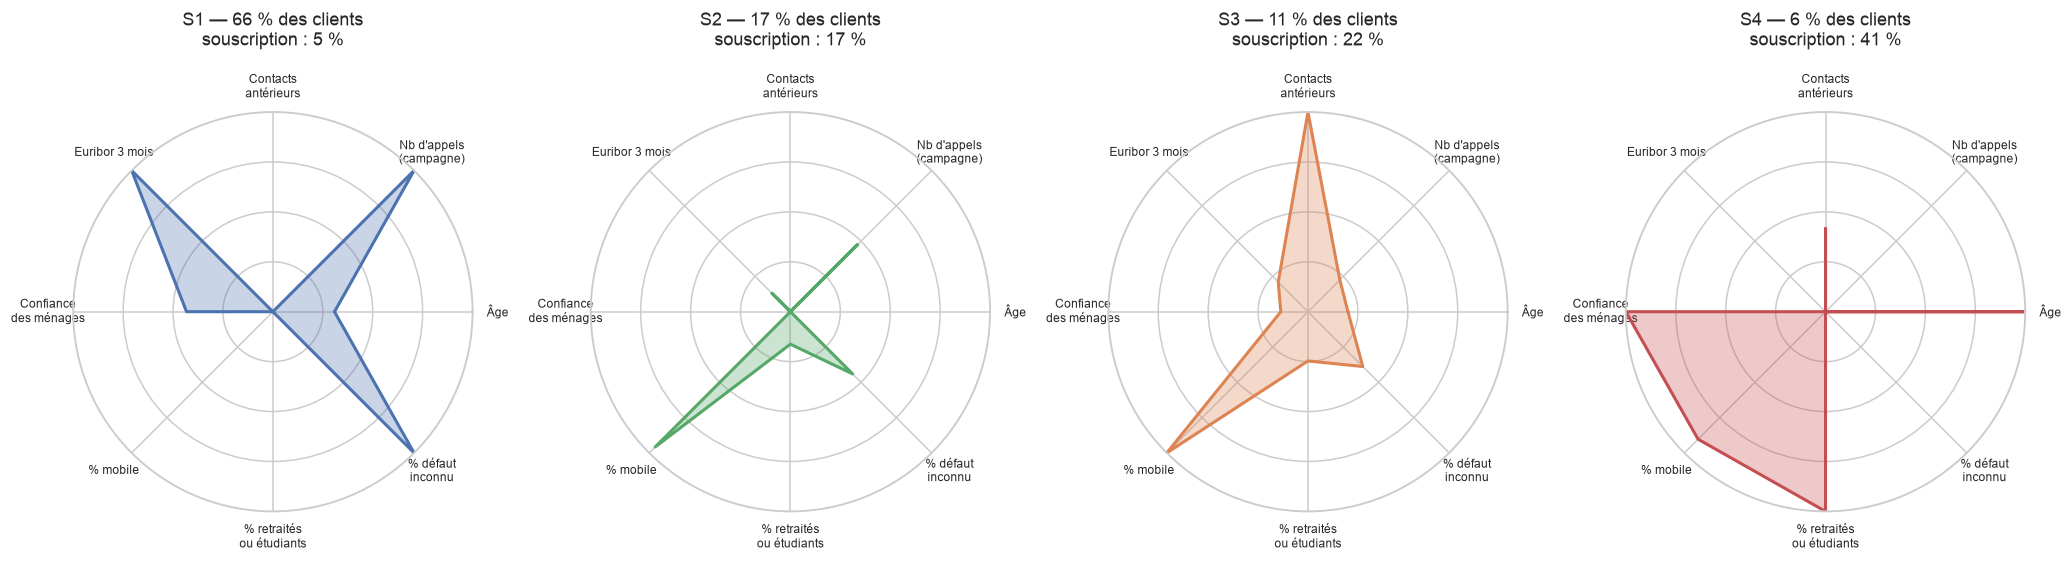
\includegraphics[width=\textwidth]{05_radars.png}
\caption{Radars des segments. Chaque indicateur est ramené entre 0 (segment le plus bas) et 1 (segment le plus haut).}\label{fig:radar}
\end{figure}

Trois dimensions structurent donc la clientèle, dans cet ordre : le \textbf{contexte économique} au moment du contact, l'\textbf{historique de la relation}, puis le \textbf{profil socio-démographique} pour S4. Les crédits détenus par le client (immobilier, personnel) ne différencient presque pas les segments.

\subsection{Ce que rapporte le ciblage}
Le taux de souscription est multiplié par plus de sept entre S1 et S4, alors que \texttt{y} n'a servi ni à construire les groupes ni à choisir la solution. En appelant les segments par ordre de priorité, S4 puis S3 puis S2, la banque contacte \textbf{33,6\,\% des clients et obtient 68,1\,\% des souscriptions}. Le taux de réussite des appels passe de 11,3\,\% à 22,8\,\%.

\subsection{Recommandations}
\begin{table}[H]\centering\small
\caption{Une recommandation par segment.}\label{tab:reco}
\begin{tabularx}{\textwidth}{|L{2.6cm}|Y|Y|}
\hline
\textbf{Segment} & \textbf{Recommandation} & \textbf{Justification}\\ \hline
S4 --- Profils réceptifs & Les appeler en premier, avec les conseillers les plus expérimentés ; offre d'épargne sécurisée orientée seniors et étudiants ; un ou deux appels suffisent. & Taux 3,6 fois supérieur à la moyenne ; segment le moins sollicité (1,8 appel).\\ \hline
S3 --- Déjà démarchés & Relance personnalisée selon le résultat précédent : proposition de renouvellement aux anciens succès, nouvel argumentaire pour les anciens échecs. & Taux double de la moyenne ; le résultat précédent est la variable qui distingue le segment.\\ \hline
S2 --- Nouveaux prospects, taux bas & Campagne d'acquisition sur mobile, concentrée sur les périodes de taux bas ; deux appels au maximum. & Taux 1,5 fois supérieur à la moyenne pour un premier contact ; joints à 91\,\% sur mobile.\\ \hline
S1 --- Nouveaux prospects, taux élevés & Réduire la pression téléphonique : plafonner à deux appels, basculer vers des canaux peu coûteux (courriel, SMS), reporter la sollicitation. & 66\,\% des appels pour 32\,\% des souscriptions ; segment le plus sollicité (2,7 appels).\\ \hline
\end{tabularx}
\end{table}

Une recommandation transversale s'ajoute : les campagnes sont beaucoup plus efficaces quand les taux sont bas. Le \textbf{calendrier} des campagnes compte autant que le choix des clients.

% ------------------------------------------------------------------ 6
\section{Extensions}\label{sec:extensions}

Cette section ne modifie pas la solution retenue. Elle mesure ce qu'elle doit au contexte économique et traite deux extensions proposées par le sujet (notebook \texttt{06\_extensions}).

\subsection{Sensibilité au contexte économique}
S1 et S2 se distinguent surtout par le taux Euribor au moment de l'appel. Pour mesurer ce que la segmentation doit à la conjoncture, nous refaisons la CAH de Ward sans les trois indicateurs de contexte (\texttt{cons.price.idx}, \texttt{cons.conf.idx}, \texttt{euribor3m}). Il reste les 12 variables qui décrivent le client et sa relation avec la banque, avec le même prétraitement et le même échantillon.

\begin{itemize}
\item \textbf{Une seule structure nette subsiste} : à $k=2$ (silhouette 0,28), elle isole les clients déjà démarchés, qui souscrivent à 25\,\%. À $k=4$, la silhouette tombe à 0,12 et la stabilité bootstrap à 0,58, contre 0,21 et 0,93 pour la solution retenue.
\item Les quatre groupes obtenus sont : les déjà démarchés (qui reproduisent presque exactement S3), des clients \textbf{sur-sollicités} (7,8 appels en moyenne pendant la campagne), des seniors souvent mariés, et des jeunes actifs souvent célibataires. L'accord avec la solution retenue est faible (ARI de 0,18).
\end{itemize}

\begin{table}[H]\centering\small
\caption{Taux de souscription des groupes « client » (sans contexte) selon la période du contact.}\label{tab:ctx}
\begin{tabular}{|l|c|c|}
\hline
\textbf{Groupe « client »} & \textbf{Taux bas (Euribor < 3\,\%)} & \textbf{Taux hauts (Euribor $\geq$ 3\,\%)}\\ \hline
Déjà démarchés      & 30,1\,\% & 3,7\,\%\\ \hline
Sur-sollicités      & 10,1\,\% & 4,4\,\%\\ \hline
Seniors             & 24,2\,\% & 4,4\,\%\\ \hline
Jeunes actifs       & 21,6\,\% & 5,3\,\%\\ \hline
Ensemble            & 24,5\,\% & 4,8\,\%\\ \hline
\end{tabular}
\end{table}

Le tableau~\ref{tab:ctx} sépare les deux effets. \textbf{Le contexte domine} : dans chaque groupe, la souscription est quatre à huit fois plus forte en période de taux bas. \textbf{À période égale, le profil compte encore}, mais surtout par l'historique et par la pression d'appels. Seniors et jeunes actifs ont des taux voisins : la démographie seule discrimine peu. Le groupe des sur-sollicités se lit avec prudence, car les appels d'une campagne s'arrêtent souvent après une souscription : beaucoup d'appels est en partie une \emph{conséquence} de la non-souscription.

\subsection{Clients atypiques (extension n\textsuperscript{o}~1)}
Deux détecteurs fondés sur des principes différents sont comparés sur l'échantillon : le \textbf{bruit de DBSCAN} (densité locale, réglages du Jour 3) et l'\textbf{Isolation Forest} (un point est atypique s'il s'isole en peu de coupures aléatoires), réglée pour signaler la même proportion de clients (3,8\,\%, soit 150).

\begin{table}[H]\centering\small
\caption{Profil des clients atypiques (échantillon de 4\,000 clients).}\label{tab:atyp}
\begin{tabular}{|l|c|c|c|c|}
\hline
 & \textbf{Bruit DBSCAN} & \textbf{Isolation Forest} & \textbf{Les deux} & \textbf{Clients ordinaires}\\ \hline
Nombre de clients          & 150 & 150 & 66 & 3\,766\\ \hline
Taux de souscription       & 49\,\% & 46\,\% & 56\,\% & 9\,\%\\ \hline
Déjà démarchés             & 42\,\% & 62\,\% & 79\,\% & 1\,\%\\ \hline
Succès précédent           & 37\,\% & 57\,\% & 70\,\% & 1\,\%\\ \hline
Retraités ou étudiants     & 34\,\% & 30\,\% & 45\,\% & 5\,\%\\ \hline
Euribor moyen              & 1,2 & 1,1 & 0,9 & 3,8\\ \hline
\end{tabular}
\end{table}

Les deux méthodes s'accordent sur 66 clients, soit 44\,\% du bruit DBSCAN (tableau~\ref{tab:atyp}). Ces atypiques ne sont pas des erreurs de saisie : ce sont surtout d'\textbf{anciens souscripteurs}, des retraités et des étudiants, contactés en période de taux bas. Ils souscrivent à près de 50\,\%, soit plus de quatre fois la moyenne, et le taux de souscription croît avec le score d'anomalie. Les méthodes de partitionnement les noient dans S3 ou S4 ; le score d'Isolation Forest permet de les extraire et de les confier en priorité aux conseillers.

\subsection{Application d'affectation (extension n\textsuperscript{o}~3)}
La règle du centre le plus proche est déployée dans une application Streamlit (\texttt{app/streamlit\_app.py}). L'utilisateur saisit les 15 variables actives d'un nouveau client. L'application l'encode avec le préprocesseur ajusté sur la population, l'affecte au segment le plus proche, puis affiche le taux de souscription observé du segment et la recommandation correspondante. Elle reproduit à 100\,\% les segments de la population calculés au Jour 5.

% ------------------------------------------------------------------ 7
\section{Discussion}

\textbf{Une structure réelle mais faible.} Avec des silhouettes autour de 0,2, les segments sont des tendances et non des catégories étanches. Ce résultat est cohérent sur toutes les méthodes et avec les projections : la clientèle forme un continuum.

\textbf{Le poids du contexte.} S1 et S2 se distinguent surtout par la période du contact, pas par ce que le client \emph{est}. Un même client appelé à un autre moment pourrait changer de segment. L'analyse de sensibilité (section~\ref{sec:extensions}) le confirme : sans le contexte, seul l'historique de contact forme un groupe net. Garder le contexte reste un choix défendable, car la banque doit décider \emph{qui} appeler et \emph{quand}, et la période est le facteur le plus prédictif. Mais S1 et S2 doivent être présentés comme des situations de contact plutôt que comme des types de clients. La segmentation est donc très utile pour planifier les campagnes, moins pour connaître les personnes. Le fichier ne contient d'ailleurs ni revenu, ni solde, ni ancienneté : la description socio-démographique reste limitée.

\textbf{Des choix de modélisation assumés.} Écarter \texttt{duration} et les variables redondantes s'éloigne du squelette fourni, mais évite de faire entrer la cible dans le clustering et de compter plusieurs fois la conjoncture. Le choix de $k=4$ répond à un besoin métier ; un statisticien pur retiendrait $k=2$.

\textbf{Ce que chaque méthode a apporté.} Aucune méthode n'est inutile. K-means et K-prototypes confirment la structure principale ; Gower montre que cette structure dépend du poids donné au contexte ; les liens \emph{average} et \emph{complete} et DBSCAN révèlent des niches et des clients atypiques ; le mélange gaussien rappelle qu'un critère comme le BIC ne vaut que si l'hypothèse du modèle tient.

\textbf{Pistes.} Comparer plusieurs méthodes de sélection de variables avant le clustering ; reproduire l'étude sur un second jeu de données (par exemple une segmentation RFM) ; enrichir le fichier client (revenu, encours, ancienneté) pour obtenir des profils moins dépendants de la conjoncture.

% ------------------------------------------------------------------ 7
\section{Conclusion}

À partir de données mixtes et sans utiliser la variable de souscription, nous avons construit une segmentation en quatre groupes par classification hiérarchique de Ward. Elle offre le meilleur compromis entre qualité statistique (silhouette 0,21 ; Davies-Bouldin 1,73), stabilité (ARI bootstrap 0,93) et besoin métier. Les segments ont des taux de souscription allant de 5\,\% à 41\,\% : un tiers des clients concentre deux tiers des souscriptions. L'analyse de sensibilité rappelle qu'une partie de cet écart tient à la période du contact. Les clients atypiques repérés par DBSCAN et l'Isolation Forest forment un petit vivier très réceptif.

Sur le plan de la méthode, trois enseignements se dégagent. La standardisation et le choix de la distance changent réellement les groupes. Un indice de qualité ne se lit jamais seul : les partitions les mieux notées en silhouette étaient ici les moins utiles. Enfin, le nombre de groupes est un compromis entre ce que disent les données et ce dont le métier a besoin, et ce compromis doit être énoncé clairement.

\section*{Références}
\begin{itemize}
\item S. Moro, P. Cortez, P. Rita (2014). \emph{A data-driven approach to predict the success of bank telemarketing}. Decision Support Systems, 62, 22--31. Jeu de données \emph{Bank Marketing}, UCI Machine Learning Repository.
\item J. C. Gower (1971). \emph{A general coefficient of similarity and some of its properties}. Biometrics, 27(4), 857--871.
\item Z. Huang (1998). \emph{Extensions to the k-means algorithm for clustering large data sets with categorical values}. Data Mining and Knowledge Discovery, 2, 283--304.
\item M. Ester, H.-P. Kriegel, J. Sander, X. Xu (1996). \emph{A density-based algorithm for discovering clusters in large spatial databases with noise}. KDD-96.
\item P. J. Rousseeuw (1987). \emph{Silhouettes: a graphical aid to the interpretation and validation of cluster analysis}. Journal of Computational and Applied Mathematics, 20, 53--65.
\item F. Pedregosa et al. (2011). \emph{Scikit-learn: Machine Learning in Python}. Journal of Machine Learning Research, 12, 2825--2830.
\item Support de cours « Apprentissage non supervisé », Master BDA/IA, UN-CHK.
\end{itemize}

\end{document}
